\chapter{Perceptual Experiments}
\label{chap:PerceptualExperiments}

\section{Reconstruction of Individual Harmonics}
\label{sec:PerceptualExperiments-Reconstruction}
	An experiment was conducted to evaluate which harmonic excitation method is best suited to the generation of
	individual harmonics. A primary aim of this experiment was to determine whether any of the methods would cause a
	tone from a single instrument to be perceived as coming from multiple sources. Each method was used to reconstruct
	signals which from which some harmonic content had been removed. The quality of the reconstruction was assessed by
	participants in a multiple stimulus listening test. 

	\note{The same stimuli from chapter 6 are used.}

	For each stimuli the third through ninth harmonics were removed. Spectrograms of the cello stimulus before and after
	this process are shown in Figures \ref{fig:CelloSpectrogram} and \ref{fig:CelloFilteredSpectrogram}.  Test stimuli
	were then created by reintroducing these harmonics using SSBA, IAP and a synthesis method.  The synthesis method
	consisted of using the STFT to measure the amplitude envelope of the fundamental frequency and applying this to a
	synthesised sine wave at the frequency of the desired harmonic. 

	\begin{figure}[h!]
		\centering
		\captionsetup[subfigure]{oneside,margin={1cm, 0cm}}
		\subfloat[Unprocessed Stimulus]
		{
			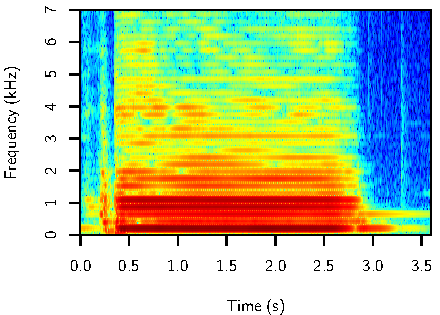
\includegraphics{chapter7/Images/CelloSpectrogram.pdf}
			\label{fig:CelloSpectrogram}
		}
		\quad
		\subfloat[Filtered Stimulus]
		{
			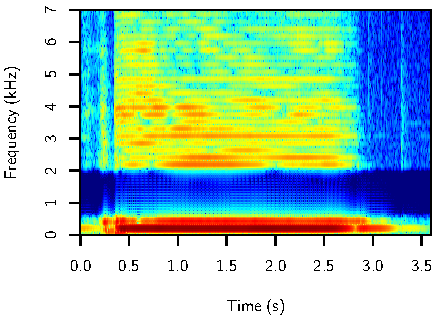
\includegraphics{chapter7/Images/CelloFilteredSpectrogram.pdf}
			\label{fig:CelloFilteredSpectrogram}
		}
		\caption{Spectrograms of the cello stimulus.}
		\label{fig:CelloSpectrograms}
	\end{figure}

	Each stimulus was reconstructed three times using each method, using different parameters each time. For the SSBA
	and IAP methods a different order FIR filter was used to isolate the fundamental frequency. The filters used had
	orders of 50, 100 and 500. For the synthesis method the window length of the STFT was changed, taking values of 50,
	100 and 500 samples. Spectrograms for the reconstructed stimuli, using the smallest filter order / STFT window
	length, are shown in Figure \ref{fig:ReconstructedCelloSpectrograms}.

	\begin{figure}[h!]
		\centering
		\captionsetup[subfigure]{oneside,margin={1cm, 0cm}}
		\subfloat[SSBA with a 50\super{th} order filter.]
		{
			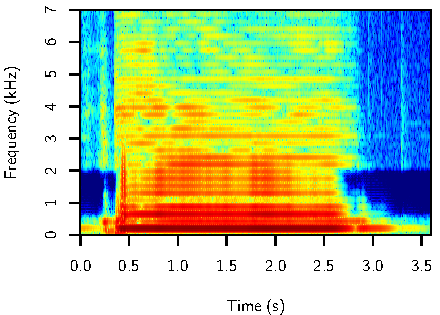
\includegraphics{chapter7/Images/CelloSSBASpectrogram.pdf}
			\label{fig:CelloSSBASpectrogram}
		}
		\quad
		\subfloat[IAP with a 50\super{th} order filter.]
		{
			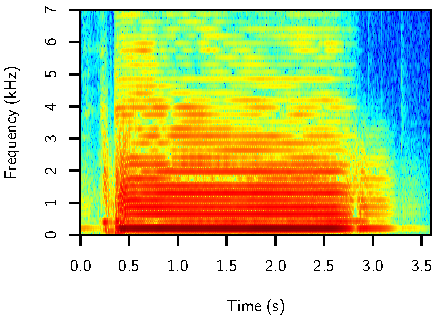
\includegraphics{chapter7/Images/CelloIAPSpectrogram.pdf}
			\label{fig:CelloIAPSpectrogram}
		}
		
		\subfloat[Synthesis with an STFT window length of 50 samples.]
		{
			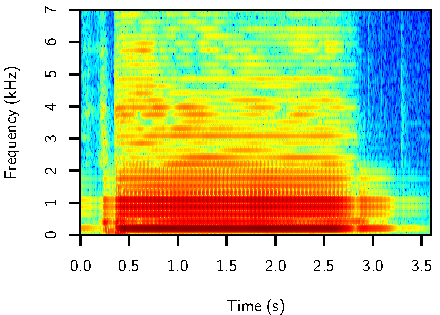
\includegraphics{chapter7/Images/CelloSynthesisSpectrogram.pdf}
			\label{fig:CelloSynthesisSpectrogram}
		}
		\caption{Spectrograms of the cello stimulus reconstructed using three different methods.}
		\label{fig:ReconstructedCelloSpectrograms}
	\end{figure}

	On inspection of these spectrograms the characteristics of the three excitation methods can be seen. The amplitude
	envelopes of the generated harmonics differ greatly between the methods. Comparing the decay portion of the
	envelopes compared with those in the original signal (Figure \ref{fig:CelloSpectrogram}) highlights these
	differences. In the cello stimulus the fundamental frequency and third harmonic have a longer decay time then the
	other harmonics. The harmonics generated by the IAP and synthesis methods (Figures \ref{fig:CelloIAPSpectrogram} and
	\ref{fig:CelloSynthesisSpectrogram}) use the amplitude envelope of the fundamental frequency extending the decay
	time of the these harmonics compared to that in the original. Those generated by the SSBA method (Figure
	\ref{fig:CelloSSBASpectrogram}) have shortened decay times. As the order of the harmonic is increased the decay time
	gets shorter due to the dynamic expansion shown in Figure \ref{fig:SSBATemporalEffects}.

	The amplitude envelopes of the harmonics generated using the synthesis techniques exhibit a large amount of ripple.
	This is due to the amplitude of the fundamental being calculated in blocks. These inaccuracies are not present in
	the harmonics generated using the IAP method as the amplitude is calculated on a sample by sample basis.

	Test participants were presented with all processed version of a particular stimulus at once along with a reference
	stimulus (the unprocessed stimulus) and an anchor stimulus (the stimulus with its harmonics removed).  Participants
	were asked to grade how well each processed stimulus recreated the reference stimulus on a scale from 0 to 100.

	The results of this experiment are shown in Figure \ref{fig:SMCResults} with error bars showing the 95\% confidence
	intervals. The stimuli numbers refer to different processing algorithms as follows.

	\begin{tabular}{>{\bfseries}rl}
		1. & The reference stimulus. \tabularnewline
		2. & Stimulus reconstructed using the synthesis method with an STFT window length of 50
		     samples. \tabularnewline
		3. & Stimulus reconstructed using the synthesis method with an STFT window length of 100
		     samples. \tabularnewline
		4. & Stimulus reconstructed using the synthesis method with an STFT window length of 500
		     samples. \tabularnewline
		5. & Stimulus reconstructed using the SSBA method using a 50\super{th} order filter. \tabularnewline
		6. & Stimulus reconstructed using the SSBA method using a 100\super{th} order filter. \tabularnewline
		7. & Stimulus reconstructed using the SSBA method using a 500\super{th} order filter. \tabularnewline
		8. & Stimulus reconstructed using the IAP method using a 50\super{th} order filter. \tabularnewline
		9. & Stimulus reconstructed using the IAP method using a 100\super{th} order filter. \tabularnewline
		10. & Stimulus reconstructed using the IAP method using a 500\super{th} order filter. \tabularnewline
		11. & Stimulus with third through ninth harmonics removed (anchor).
	\end{tabular}

	\begin{figure}[h!]
		\centering
		\captionsetup[subfigure]{oneside,margin={1cm, 0cm}}
		\subfloat[Cello Stumulus]
		{
			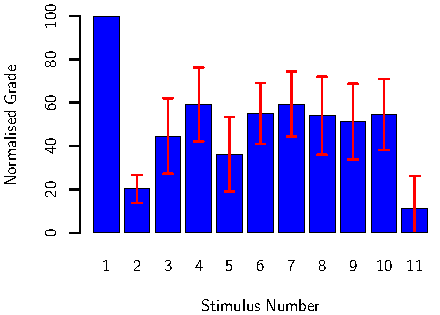
\includegraphics{chapter7/Images/CelloResults.pdf}
			\label{fig:CelloResults}
		}
		\quad
		\subfloat[Clarinet Stimulus]
		{
			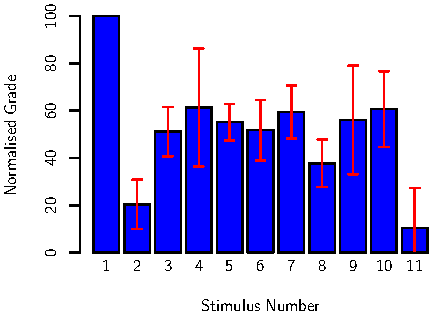
\includegraphics{chapter7/Images/ClarinetResults.pdf}
			\label{fig:ClarinetResults}
		}

		\subfloat[Synthesised Stimulus]
		{
			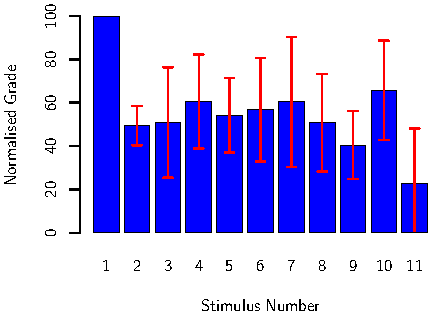
\includegraphics{chapter7/Images/SynthResults.pdf}
			\label{fig:SynthResults}
		}
		\quad
		\subfloat[Piano Stimulus]
		{
			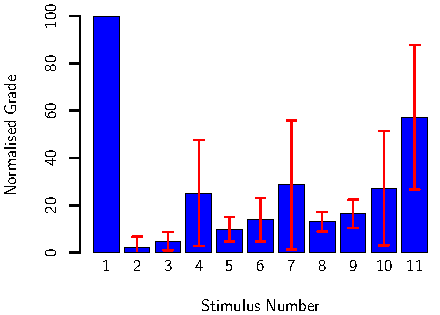
\includegraphics{chapter7/Images/PianoResults.pdf}
			\label{fig:PianoResults}
		}
		\caption{Mean grades and confidence intervals for each of the stimuli.}
		\label{fig:SMCResults}
	\end{figure}

	Across all the stimuli there is a general increase in the perceived quality of the reproduction as the filter order
	or STFT window length is increased. With the SSBA and IAP methods increasing the filter order increases the level
	difference between the fundamental and its harmonics, better isolating the fundamental.  This is turn reduces the
	levels of intermodulation distortion in the output producing a `cleaner' harmonic.  With the synthesis method
	increasing the STFT window length increases the frequency resolution allowing for the amplitude envelope of the
	fundamental frequency to be measured more precisely.

	The piano stimulus used had very little energy at its fundamental frequency. This illustrates the problem discussed
	previously, there is not enough information in the amplitude envelope of the fundamental to reproduce the other
	harmonics. This leads to much lower grades for the reproduced signals than for any of the other stimuli. Figure
	\ref{fig:PianoResults} shows that the piano stimulus with its harmonics missing received a higher grade on average
	then any of the reconstructed stimuli further showing how poor the quality of the reconstructions is.

	The confidence intervals for the grades given to the majority of the stimuli are high. This is most likely due to
	there being too few participants in the experiment. To supplement these results each of the stimuli was graded with
	the R\sub{nonlin} metric. These results were normalised to the same range as the results from the listening test and
	are displayed in Figure \ref{fig:SMCRNonlin}.

	\begin{figure}[h!]
		\centering
		\captionsetup[subfigure]{oneside,margin={1cm, 0cm}}
		\subfloat[Cello Stimulus]
		{
			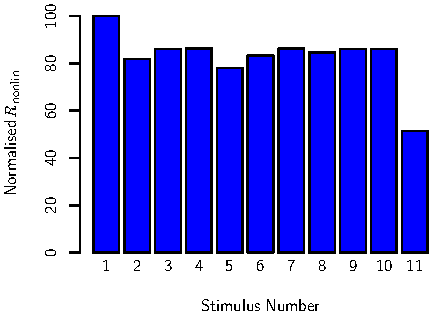
\includegraphics{chapter7/Images/CelloRNonlin.pdf}
			\label{fig:CelloRNonlin}
		}
		\quad
		\subfloat[Clarinet Stimulus]
		{
			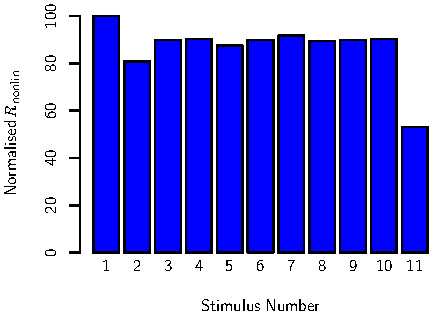
\includegraphics{chapter7/Images/ClarinetRNonlin.pdf}
			\label{fig:ClarinetRNonlin}
		}

		\subfloat[Synthesised Stimulus]
		{
			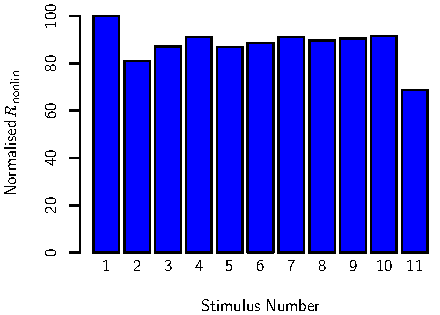
\includegraphics{chapter7/Images/SynthRNonlin.pdf}
			\label{fig:SynthRNonlin}
		}
		\quad
		\subfloat[Piano Stimulus]
		{
			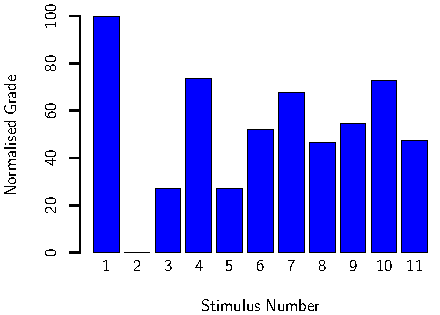
\includegraphics{chapter7/Images/PianoRNonlin.pdf}
			\label{fig:PianoRNonlin}
		}
		\caption{R\sub{nonlin} values for each of the stimuli.}
		\label{fig:SMCRNonlin}
	\end{figure}

	The R\sub{nonlin} values support the correlations found in the listening test results. Using a higher order filter
	to isolate the fundamental improves the quality of the reconstruction. Figure \ref{fig:PianoRNonlin} again
	illustrates the problems which arise when the input signal has little energy at its fundamental frequency. Several
	of the reconstructions are objectively less similar to the original stimulus than the anchor stimulus is.

	Both sets of results show that, using the highest order filter / STFT window lengths, each of the methods produce
	similar quality reconstructions of the original signal. For shorter filter lengths the IAP method provides more
	quality at then the SSBA method at the expense of requiring slightly more computation. The synthesis method produces
	similar quality results but incurs further computational complexity. 

	For timbral control applications the IAP method provides the greatest flexibility. For the majority of stimuli in
	this experiment it reproduced signals with the highest perceived quality. It was also shown in section
	\ref{sec:ExcitationEvaluation-Comparison-Homogeneity} that it is a homogeneous process allowing it to be applied to
	a wider range of signals with more predictable effects.

\section{Semantic Control}
\label{sec:PerceptualExperiments-SemanticControl}
	\note
	{
		Why these descriptors (most agreed upon clusters from chapter 4, harsh not agreed upon but seems to be
		related to bright so kept in to test how well it will perform).

		Reorganise to a paper style 1. intro 2. system design 3. testing methodology 4. results 5. discussion
		do similar with the above experiment.
	}

	The findings of Chapter \ref{chap:TimbreEvaluation} can be combined with the techniques discussed in Chapter
	\ref{chap:FeatureControl} to develop audio effects with control parameters which relate to specific descriptive
	terms. In this section two such effects are developed and their performance evaluated. Each of these effects have a
	single `semantic' control parameter which changes processing parameters based three related semantic terms. The
	first effect, the warmth / harshness effect, is intended to introduce `warmth' for low values of the
	control parameter, `brightness' for middle values of the control parameter and `harshness' for high values of the
	control parameter. The second effect, the harshness / crunchiness effect, is intended to change between
	`harshness', `brightness' and `crunchiness' for different values of the control parameter.

	The performance of each effect is evaluated using a set of ten test signals, comprising two electric bass guitars
	(B1 and B2), a flute (F), two electric guitars (G1 and G2), a marimba (M), an oboe (O), a saxophone (S), a trumpet
	(T) and a violin (V). The signals were adjusted to have equal loudness prior to experimentation.  Firstly the
	effects are evaluated objectively by comparing them to the analysis performed in Chapter
	\ref{chap:TimbreEvaluation}. Secondly the effects are evaluated subjectively as discussed in Sections
	\ref{sec:PerceptualExperiments-SemanticControl-EvaluationExperiment} and
	\ref{sec:PerceptualExperiments-SemanticControl-PerformanceResults}.

	\subsection{Semantically Controlled Effect Design}
	\label{sec:PerceptualExperiments-SemanticControl-EffectDesign}
		This section describes the underlying systems of the warmth / harshness and harshness / crunchiness effects
		and the operation of their control parameters. The performance of each effect is evaluated objectively by
		examining how they manipulate the features of the test signals. Each effect is used to process each of the
		test signals with its parameter set to the minimum value, the middle value and the maximum value,
		corresponding to `warm', `bright' and `harsh' for the warmth / harshness effect and `harsh', `bright' and
		`crunchy' for the harshness / crunchiness effect. The audio features of the unprocessed and processed
		signals in each of these applications are calculated in the same manner as in the SAFE plug-ins. These audio
		features are the compared to those taken from the SAFE dataset.

		As discussed in Chapter \ref{chap:TimbreEvaluation} the terms `warm', `harsh' and `bright' are all used to
		describe transformations applied by both distortion and equalisation effects. `Harsh' and `bright' having
		different definitions depending on the type of processing applied. The objective performance of the effects
		proposed in this section is evaluated against data from both the SAFE distortion and equaliser. In order to
		do this, two new timbre spaces are constructed by performing PCA on the processed audio features and feature
		differences of the combined distortion and equaliser data. Two performance scores are given to each
		combination of audio effect, descriptor and test signal. The first measuring how close the processed
		features of the signal are to points labelled with the descriptor in the processed feature timbre space.
		The second measuring how close the changes in features caused by the effect are to points labelled with the
		descriptor in the feature difference timbre space.

		The performance of a particular effect, with a particular parameter setting on a particular test signal is
		measured by projecting the extracted audio features to a point on the relevant timbre space. The processed
		features of the signal are projected onto the processed feature timbre space and the feature differences
		onto the feature difference timbre space. The Mahalanobis distance, $M(x, d)$, between this point, $x$, and
		the distribution of transforms labelled with the descriptor, $d$, is taken using Equation
		\ref{eq:Mahalanobis}
		
		\begin{equation}
			M(x, d) = \sqrt{(x - \mu_{d})^{T}\Sigma_{d}^{-1}(x - \mu_{d})}
			\label{eq:Mahalanobis}
		\end{equation}

		Where $x$ is a column vector containing the coordinates of the point in the timbre space, $\mu_{d}$ a column
		vector containing the mean coordinates of all transforms in the timbre space labelled with descriptor $d$
		and $\Sigma_{d}$ the covariance matrix of those transforms' coordinates in the timbre space. The number of
		coordinates used in the calculation of Mahalanobis distance is determined in the same manner as discussed in
		Section \ref{sec:TimbreEvaluation-Analysis-Agreement}. Where there more than five transforms in the
		distribution, the coordinates in the first five PCs of the timbre space are used. Where the number of points
		in the distribution, $N_{d}$, is lower, only the first $N_{d} - 1$ coordinates can be used in order to avoid
		$\Sigma_{d}$ being singular.

		Where the descriptor, $d$, is represented by two distributions of transforms, one from the distortion and
		one from the equaliser, the Mahalanobis distance from both distributions is taken and the minimum distance
		kept as the measure of performance.

		\subsubsection*{Warmth / Harshness}
			The warmth / harshness effect controls the spectral centroid of a signal using a refined version of
			the system given in Figure \ref{fig:TwoBandSpectralCentroidSystem}. Two spectral bands are
			generated, one with a spectral centroid lower than the input signal and one with a higher spectral
			centroid than the input signal. The relative levels of these bands is then adjusted in order to
			adjust the output's spectral centroid. The full system is shown in Figure \ref{fig:WarmHarsh}.

			\begin{figure}[h!]
				\centering
				\begin{tikzpicture}
					\node (In) at (-1, -3.25) {$x[n]$};
					\coordinate (InMid) at (0, -3.25);
					\draw (In) -- (InMid);

					\coordinate (Side1) at (0, -1.25);
					\coordinate (Side2) at (0, -2.25);
					\draw (InMid) -- (Side2);
					\draw (Side2) -- (Side1);

					\node (F0) [draw] at (2, -1.25) {$f_{0}$ Tracker};
					\node (F0Filter) [draw] at (2, -2.25) {LPF};
					\draw (Side2) -- (F0Filter);
					\draw (F0) -- (F0Filter);
					\draw (Side1) -- (F0);

					\node (Centroid) [draw] at (2, -3.25) {$\mu_{s}$ Tracker};
					\draw (InMid) -- (Centroid);

					\node (Add) [operator] at (10.5, -3.25) {+};

					% NLD
					\node (NLD) [draw] at (4.5, -2.25) {Full Wave Rectifier};
					\draw (F0Filter) -- (NLD);

					\node (NLDFilter) [draw] at (7, -2.25) {HPF};
					\draw (NLD) -- (NLDFilter);

					\node (NLDGain) [gain, minimum size=1.7cm] at (8.5, -2.25) {$m_{H}$};
					\draw (NLDFilter) -- (NLDGain);
					\coordinate (NLDOut) at (9.5, -2.25);
					\draw (NLDGain) -- (NLDOut);
					\draw (NLDOut) -- (Add);

					\coordinate (NLDSide) at (7, -3.25);
					\draw (Centroid) -- (NLDSide);
					\draw (NLDSide) -- (NLDFilter);

					% through
					\coordinate (Through) at (0, -4.25);
					\node (ThroughFilter) [draw] at (2, -4.25) {LPF};
					\draw (Through) -- (ThroughFilter);
					\draw (Side2) -- (Through);
					\draw (Centroid) -- (ThroughFilter);
					\node (ThroughGain) [gain, minimum size=1.7cm] at (8.5, -4.25) {$m_{L}$};
					\coordinate (ThroughOut) at (9.5, -4.25);
					\draw (ThroughFilter) -- (ThroughGain);
					\draw (ThroughGain) -- (ThroughOut);
					\draw (ThroughOut) -- (Add);

					\node (Out) at (11.75, -3.25) {$y[n]$};
					\draw (Add) -- (Out);
				\end{tikzpicture}
				\caption{The system employed in the warmth / harshness effect.}
				\label{fig:WarmHarsh}
			\end{figure}

			The low frequency band is generated by low pass filtering the input signal at its spectral centroid.
			The high frequency band is generated by applying full wave rectification to the isolated fundamental
			of the input signal and high pass filtering at the input's spectral centroid. Separating the bands
			at the spectral centroid in this way ensures that their respective spectral centroids sit either
			side of the input's. Full wave rectification is used to ensure the system is homogeneous.

			The parameter of the effect controls the relative gains applied to each of the spectral bands. The
			parameter value, $p$, ranges from 0 to 1 and is used to calculate the gains, $m_{L}$ and $m_{H}$,
			applied to the low and high frequency bands using Equation \ref{eq:WarmHarshParam}.

			\[ m_{L} = p^{3} \]
			\begin{equation}
				m_{H} = 1 - m_{L}
				\label{eq:WarmHarshParam}
			\end{equation}

			When $p = 0$  the output is a low pass filtered version of the input signal resulting in a lower
			spectral centroid than the input. This corresponds to transforms  described as `warm' in the SAFE
			dataset. When $p = 1$ the output signal consists primarily of high order harmonics resulting in an
			increase in spectral centroid and corresponding to transforms labelled `harsh' in the SAFE dataset.
			The power to which $p$ is raised was determined experimentally such that when $p = 0.5$ the effect
			applies processing which corresponds to that described as `bright' in the SAFE dataset. 

			The Mahalanobis distances between the test signals after being processed by this effect and those in
			the timbre space constructed from the SAFE dataset are shown in Figure \ref{fig:HarshJeffs}. The
			distances in the processed feature space (Figure \ref{fig:HarshProcJeff}) are not as significant as
			those in the feature difference space (Figure \ref{fig:HarshDiffJeff}) as it was determined in
			Chapter \ref{chap:TimbreEvaluation} that the descriptors `warm', `bright' and `harsh' are best
			defined by relative changes in audio feature rather than absolute values.

			\begin{figure}[h!]
				\centering
				\captionsetup[subfigure]{oneside,margin={1cm, 0cm}}
				\subfloat[Processed Featues]
				{
					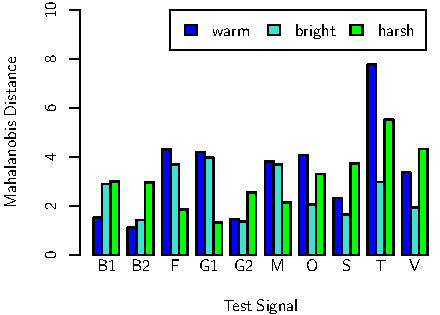
\includegraphics{chapter7/Images/HarshProcessedJeffsDistance.pdf}
					\label{fig:HarshProcJeff}
				}
				\quad
				\subfloat[FeatureDifferences]
				{
					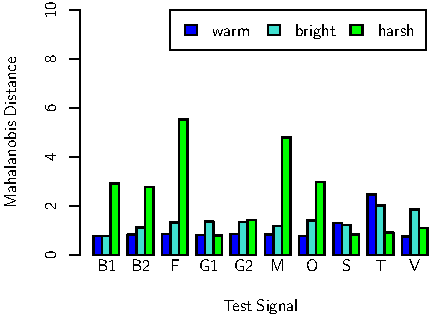
\includegraphics{chapter7/Images/HarshDifferenceJeffsDistance.pdf}
					\label{fig:HarshDiffJeff}
				}
				\caption{Mahalanobis distances for the warmth / harshness effect.}
				\label{fig:HarshJeffs}
			\end{figure}

			The results in Figure \ref{fig:HarshDiffJeff} imply that the effect is successful in applying
			transforms similar to those described as `warm' and `bright' in the SAFE dataset to a range of input
			signals. The trumpet signal poses more of a problem then the others for these descriptors. When
			attempting to make the test signals `harsher' however, the effect does not perform well on the bass
			guitar, flute, marimba or oboe signals. This is likely due to the small number of transforms
			labelled harsh in the timbre space. In Chapter \ref{chap:TimbreEvaluation} `harsh' was given a low
			agreement score in both the distortion and equaliser timbre spaces due to there only being four
			transforms labeled `harsh' in each space. As such, only a small region of the timbre space is
			described as harsh, making it more difficult design a transform which will sit in that region for a
			wide range of input signals.

		\subsubsection*{Harshness / Crunchiness}
			In Chapter \ref{chap:TimbreEvaluation} it was suggested that `crunchiness' is associated with a
			small increase in spectral irregularity and an output signal with a low spectral kurtosis and
			spectral skewness. To attempt to recreate this the harshness / crunchiness effect controls the
			spectral irregularity of a signal along with the proportion of high frequency energy introduced. The
			system is based on that described in Figure \ref{fig:SpectralShapingSystem}. The full system is
			shown in Figure \ref{fig:HarshCrunch}.

			\begin{figure}[h!]
				\centering
				\begin{tikzpicture}
					\node (In) at (-1, -1.85) {$x[n]$};
					\coordinate (InMid) at (0, -1.85);
					\draw (In) -- (InMid);

					\coordinate (Side) at (0, -0.85);
					\draw (InMid) -- (Side);

					\node (F0) [draw] at (2, -0.85) {$f_{0}$ Tracker};
					\node (F0Filter) [draw] at (2, -1.85) {LPF};
					\draw (InMid) -- (F0Filter);
					\draw (F0) -- (F0Filter);
					\draw (Side) -- (F0);

					\node (Add) [operator] at (12.5, -1.85) {+};

					\coordinate (ExciterIn) at (4, -1.85);
					\draw (F0Filter) -- (ExciterIn);

					% the fundamental
					\coordinate (F0In) at (4, 1);
					\node (F0Gain) [gain, minimum size=1.7cm] at (10, 1) {$m_{1}$};
					\draw (F0In) -- (F0Gain);
					\coordinate (F0Out) at (11, 1);
					\draw (F0Gain) -- (F0Out);
					\draw (F0Out) -- (Add);

					% second harmonic
					\coordinate (F1In) at (4, -0.7);
					\draw (F0In) -- (F1In);
					\node (F1) [draw] at (6, -0.7) {2\super{nd} Harmonic};
					\draw (F1In) -- (F1);

					\node (F1Filter) [draw] at (8.5, -0.7) {BPF};
					\draw (F1) -- (F1Filter);

					\node (F1Gain) [gain, minimum size=1.7cm] at (10, -0.7) {$m_{2}$};
					\draw (F1Filter) -- (F1Gain);
					\coordinate (F1Out) at (11, -0.7);
					\draw (F1Gain) -- (F1Out);
					\draw (F1Out) -- (Add);

					% sixth harmonic
					\coordinate (F5In) at (4, -3);
					\draw (F1In) -- (F5In);
					\node (F5) [draw] at (6, -3) {6\super{th} Harmonic};
					\draw (F5In) -- (F5);

					\node (F5Filter) [draw] at (8.5, -3) {BPF};
					\draw (F5) -- (F5Filter);

					\node (F5Gain) [gain, minimum size=1.7cm] at (10, -3) {$m_{6}$};
					\draw (F5Filter) -- (F5Gain);
					\coordinate (F5Out) at (11, -3);
					\draw (F5Gain) -- (F5Out);
					\draw (F5Out) -- (Add);

					\draw [dots] (F1) -- (F5);
					\draw [dots] (F1Filter) -- (F5Filter);
					\draw [dots] (F1Gain) -- (F5Gain);

					% high order harmonics
					\coordinate (HighIn) at (4, -4.7);
					\draw (F5In) -- (HighIn);
					\node (High) [draw] at (6, -4.7) {Full Wave Rectifier};
					\draw (HighIn) -- (High);

					\node (HighFilter) [draw] at (8.5, -4.7) {HPF};
					\draw (High) -- (HighFilter);

					\node (HighGain) [gain, minimum size=1.7cm] at (10, -4.7) {$m_{H}$};
					\draw (HighFilter) -- (HighGain);
					\coordinate (HighOut) at (11, -4.7);
					\draw (HighGain) -- (HighOut);
					\draw (HighOut) -- (Add);

					\node (Out) at (13.75, -1.85) {$y[n]$};
					\draw (Add) -- (Out);
				\end{tikzpicture}
				\caption{The system employed in the harshness / crunchiness effect.}
				\label{fig:HarshCrunch}
			\end{figure}

			Each of the individual harmonics are generated using the IAP technique discussed in Section
			\ref{sec:Excitation-Methods-IAP}. This method was chosen due to it performing the best in the
			experiments in Section \ref{sec:PerceptualExperiments-Reconstruction}. To reduce computational load
			the filter used to isolate the fundamental in this system is a second order IIR low pass filter.
			The use of a low order filter means that there is a higher proportion of high frequency energy which
			remains in the isolated fundamental. This in turn produces more intermodulation components in the
			generated harmonics. Each of the generated harmonics is band pass filtered in order to reduce the
			influence of these intermodulation components. For higher order harmonics this band pass filtering
			is not effective so only the first six harmonics are generated individually. Again a high frequency
			spectral band is generated by full wave rectifying the isolated fundamental. This high frequency
			band is high pass filtered at the frequency of the sixth harmonic so as not to interfere with the
			individually generated harmonics.

			The effect has one control parameter which ranges from 0 to 1 and controls the relative amplitudes
			of regions of the output spectrum. The spectral irregularity is controlled by adjusting the
			relative levels of the first six harmonics. The analysis and resynthesis technique discussed in
			Section \ref{sec:FeatureControl-Parameterisation-Irregularity} proved to complex to run accurately
			in real time. In its place a simpler system based on a predefined set of harmonic amplitudes,
			$c$, was used. The relative amplitudes of the harmonics are altered as the parameter value, $p$,
			is changed according to Equation \ref{eq:HarshCrunchAmps}.

			\begin{equation}
				a_{n} = p(c_{n} - 1) + 1
				\label{eq:HarshCrunchAmps}
			\end{equation}

			When $p = 0$ the first six harmonics all have the same amplitude, giving the lowest spectral
			irregularity. When $p = 1$ the relative amplitudes of the fort six harmonics are as defined by $c$.
			The values in $c$ are taken from a guitar signal, which had been processed by the SAFE distortion,
			with a Krimphoff irregularity similar to the processed signals in the SAFE dataset described as
			`crunchy'. As the parameter value is increased the spectral irregularity of the first six harmonics
			increases towards that of a `crunchy' signal. This models the increases in spectral irregularity
			noted for the transforms labelled `crunchy' in Chapter \ref{chap:TimbreEvaluation}.
			
			The relative amount of high frequency content in the output is also controlled by $p$. This is
			achieved by changing the relative levels of the band containing the first six harmonics and the band
			generated by the full wave rectifier. The final gains applied to the six generated harmonics along
			with that applied to the rectifier output are given by Equation \ref{eq:HarshCrunchParam}.

			\[ m_{n} = a_{n}\frac{3p + 2}{4} \]
			\begin{equation}
				m_{H} = \frac{8 - 7p}{5}
				\label{eq:HarshCrunchParam}
			\end{equation}

			The constants used here were derived experimentally such that when $p = 1$ the amount of energy in
			the high and low bands of the spectrum are roughly equal for a range of input signals. This produces
			the low spectral kurtosis and spectral skewness noticed in signals labeled `crunchy' in the SAFE
			dataset. Lower values of $p$ increase the levels of high frequency energy in the output signal
			causing the spectral transformations associated with `bright' and `harsh' signals.

			The Mahalanobis distances between the test signals after being processed by this effect and those in
			the timbre space constructed from the SAFE dataset are shown in Figure \ref{fig:CrunchJeffs}. Here
			both the processed features and feature differences (Figures \ref{fig:CrunchProcJeff} and
			\ref{fig:CrunchDiffJeff}) are significant as `crunchiness' is characterised by a certain change in
			spectral irregularity and the distribution of energy in the output spectrum.

			\begin{figure}[h!]
				\centering
				\captionsetup[subfigure]{oneside,margin={1cm, 0cm}}
				\subfloat[Processed Featues]
				{
					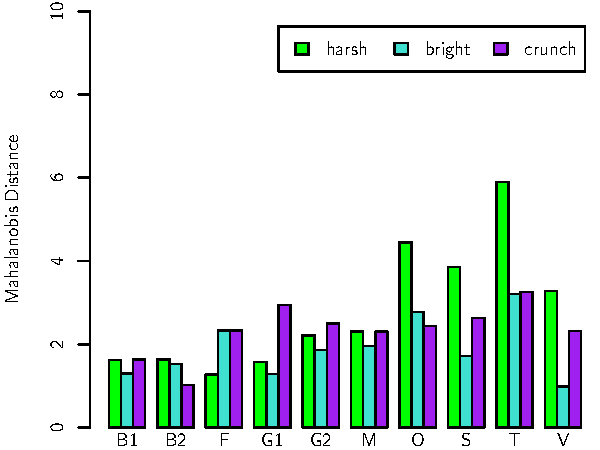
\includegraphics{chapter7/Images/CrunchProcessedJeffsDistance.pdf}
					\label{fig:CrunchProcJeff}
				}
				\quad
				\subfloat[FeatureDifferences]
				{
					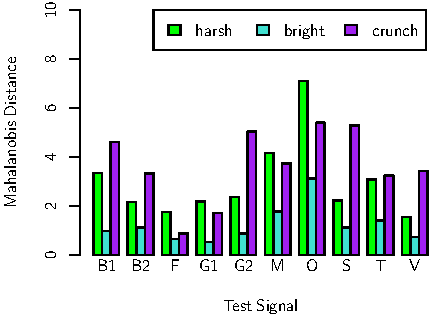
\includegraphics{chapter7/Images/CrunchDifferenceJeffsDistance.pdf}
					\label{fig:CrunchDiffJeff}
				}
				\caption{Mahalanobis distances for the harshness / crunchiness effect.}
				\label{fig:CrunchJeffs}
			\end{figure}

			Figure \ref{fig:CrunchProcJeff} shows that the effect is reasonably successful in generating output
			signals with features similar to those in the SAFE dataset labelled as `harsh', `bright' and
			`crunchy'. In, replicating the transforms which produced these signals the effect is less
			successful. This is possibly explain by the simplifications made to reduce the effects computational
			complexity. Using lower order filters increases the level of intermodulation components in the
			individually generated harmonics. Controlling the relative levels of these generated harmonics no
			longer has the expected effect on spectral irregularity as each generated harmonic contains several
			spectral partials with unknown amplitudes.

	\subsection{Evaluation Experiment}
	\label{sec:PerceptualExperiments-SemanticControl-EvaluationExperiment}
		To assess the performance of the developed effects subjectively a series of perceptual listening tests were
		undertaken. Each of the effects were implemented as audio plug-ins with the interface shown in Figure
		\ref{fig:TestPlugInterface}.

		\begin{figure}[h!]
			\centering
			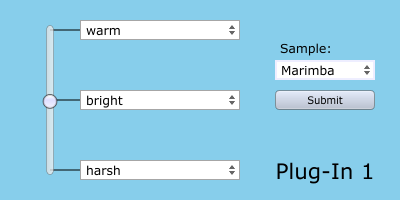
\includegraphics{chapter7/Images/TestPlugInInterface.png}
			\caption{The interface used for assessing the performance of the developed effects.}
			\label{fig:TestPlugInterface}
		\end{figure}

		\note
		{
			Randomness, DAW, list of descriptors, 3 points labelled, asked to listen to the effect prior to
			annotation.

			(airy, boomy, boxy, bright, clear, creamy, crunchy, deep, full, fuzzy, harsh, muddy, raspy, smooth,
			thin, tinny and warm)
		}

	\subsection{Performance Results}
	\label{sec:PerceptualExperiments-SemanticControl-PerformanceResults}
		\note{Cophenetic distance.}

		\begin{figure}[h!]
			\centering
			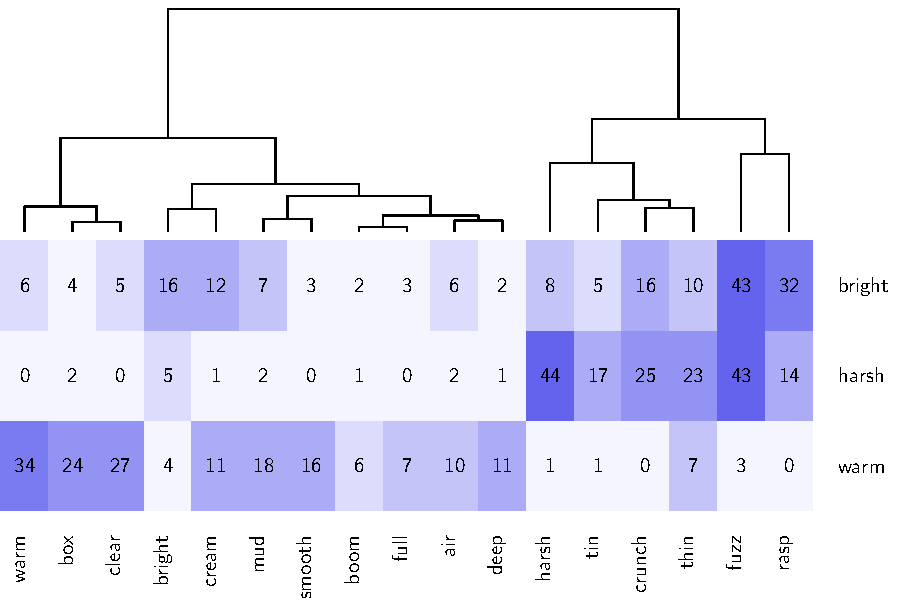
\includegraphics{chapter7/Images/HarshConfusion.pdf}
			\caption{Heat map of term usage for the warmth / harshness effect.}
		\end{figure}

		\begin{figure}[h!]
			\centering
			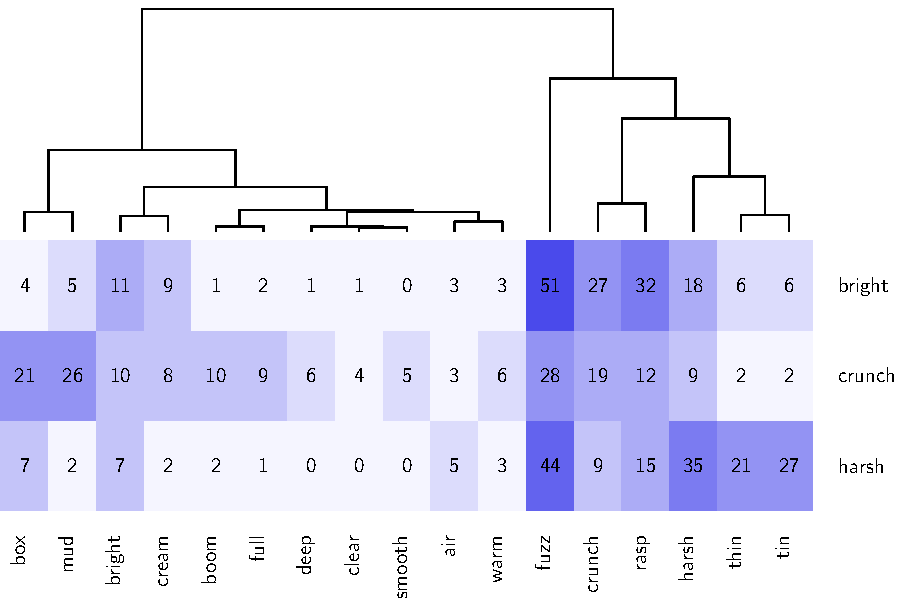
\includegraphics{chapter7/Images/CrunchConfusion.pdf}
			\caption{Heat map of term usage for the harshness / crunchiness effect.}
		\end{figure}

		\begin{figure}[h!]
			\centering
			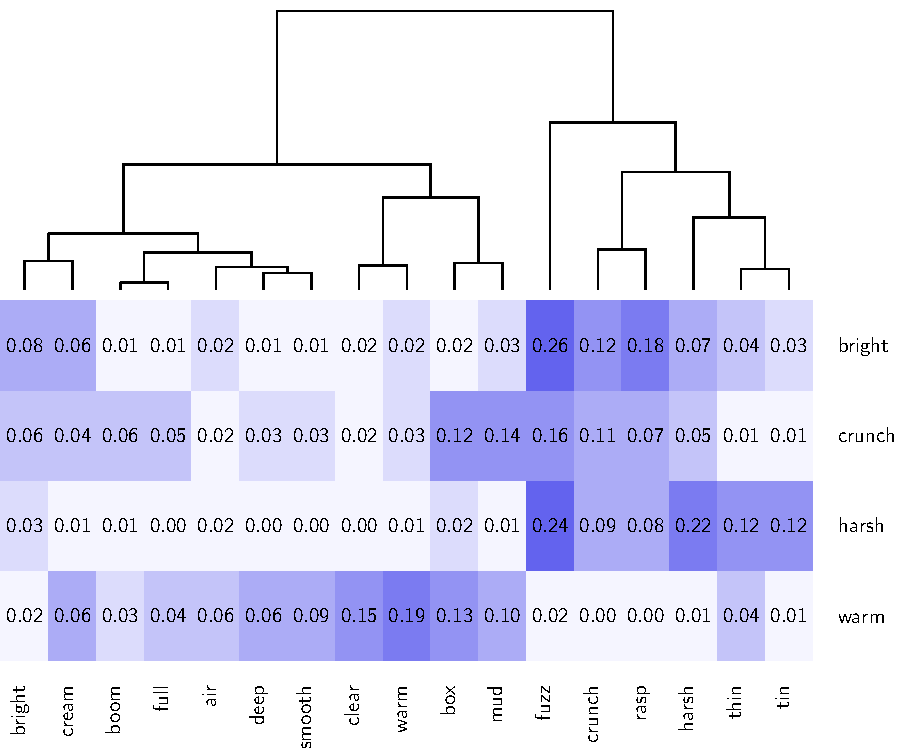
\includegraphics{chapter7/Images/CombinedConfusion.pdf}
			\caption{Heat map of term usage across both effects.}
		\end{figure}

		\begin{figure}[h!]
			\centering
			\captionsetup[subfigure]{oneside,margin={1cm, 0cm}}
			\subfloat[Processed Featues]
			{
				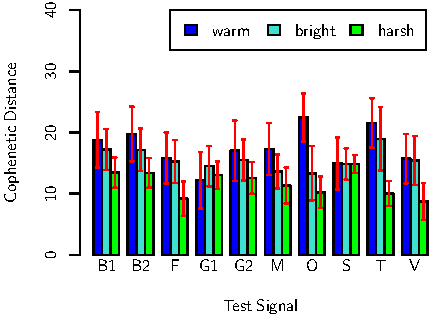
\includegraphics{chapter7/Images/HarshProcessedCophDistance.pdf}
				\label{fig:HarshProcCoph}
			}
			\quad
			\subfloat[FeatureDifferences]
			{
				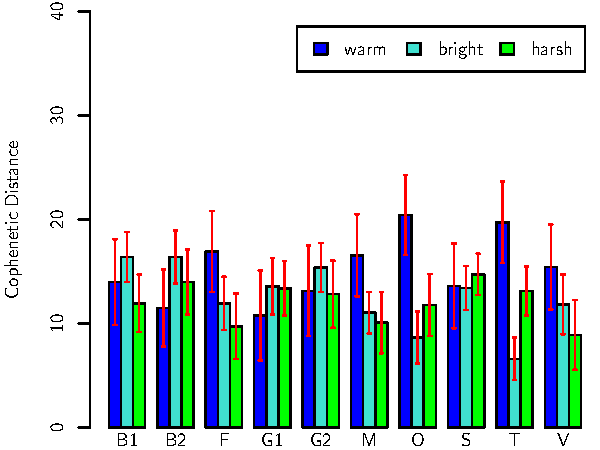
\includegraphics{chapter7/Images/HarshDifferenceCophDistance.pdf}
				\label{fig:HarshDiffCoph}
			}
			\caption{Cophenetic distances for the warmth / harshness effect.}
			\label{fig:HarshCophs}
		\end{figure}

		\begin{figure}[h!]
			\centering
			\captionsetup[subfigure]{oneside,margin={1cm, 0cm}}
			\subfloat[Processed Featues]
			{
				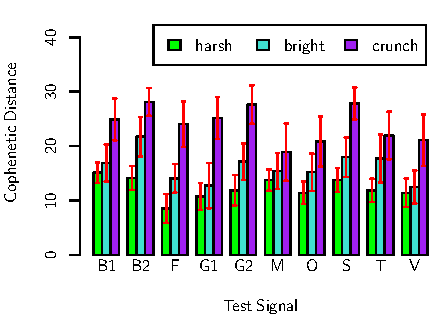
\includegraphics{chapter7/Images/CrunchProcessedCophDistance.pdf}
				\label{fig:CrunchProcCoph}
			}
			\quad
			\subfloat[FeatureDifferences]
			{
				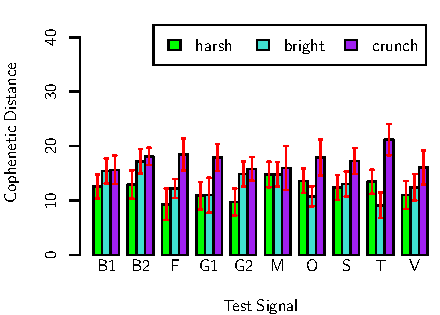
\includegraphics{chapter7/Images/CrunchDifferenceCophDistance.pdf}
				\label{fig:CrunchDiffCoph}
			}
			\caption{Cophenetic distances for the harshness / crunchiness effect.}
			\label{fig:CrunchCophs}
		\end{figure}
